% Capíulo 5
\chapter{Trabalhos Relacionados} \label{ch:trabalhos-relacionados}

Este capítulo confronta este trabalho com outras pesquisas que analisam a evolução do desempenho de sistemas. Qualquer trabalho ou ferramenta que mensure a evolução do atributo de qualidade de desempenho e possua visualizações para exibi-la é considerado relacionado a este. Na seção \ref{sec:trabalhos-relacionados-ferramentas-profiling} são comentadas as ferramentas de \textit{profiling}. Na seção \ref{sec:trabalhos-relacionados-ferramentas-apm} são mostradas as ferramentas APM. Por fim, na seção \ref{sec:trabalhos-relacionados-adordagens-degradacao-desempenho} são discutidas as abordagens de medição da degradação de desempenho.

Muitas abordagens relacionadas a visualização de software têm sido propostas para comparar versões de software de um ponto de vista geral da arquitetura \cite{Steinbruckner2010b}\cite{Telea2008}\cite{Collberg2003}\cite{Eick1992}\cite{Holten2008}. Outras abordagens focam em visualizar as métricas do software em diferentes versões \cite{Langelier2008}\cite{Lanza2001}\cite{Pinzger2005}\cite{Wettel2008}. No entanto, essas abordagens diferem deste trabalho uma vez que o objetivo é comparar um aspecto dinâmico do software, o desempenho, ao invés de aspectos estáticos ou estruturais.

\section{Ferramentas de Profiling} \label{sec:trabalhos-relacionados-ferramentas-profiling}

Há ferramentas de \textit{profiling} que podem realizar a medição do atributo de qualidade de desempenho, no entanto, com diferentes características. A \textit{VisualVM} \cite{Vis} exibe o tempo de execução de cada método e o usuário pode, à medida que deseja, tirar fotografias instantâneas da execução do software, os chamados \textit{snapshots}. Essa ferramenta, no entanto, não oferece a comparação do tempo de execução do mesmo método em versões anteriores do software, tornando difícil a visualização da evolução do atributo de qualidade de desempenho, uma vez que teria que ser feita manualmente para cada método desejado.

O \textit{JProfiler} \cite{JProfiler}, ferramenta paga, pode exibir o grafo de chamadas dos métodos, com seus respectivos tempos de execução. Assim como o \textit{VisualVM}, a ferramenta oferece a possibilidade de guardar \textit{snapshots} de determinados momentos da execução. Contudo, esses \textit{snapshots} não são automáticos, o usuário precisa, deliberadamente, informar à ferramenta quando ele deve ser acionado. Uma maneira de contornar esse problema é fazendo o uso de \textit{triggers}, onde o usuário pode configurar a ferramenta para responder a determinados eventos da JVM e, assim, executar algumas ações. Apesar da funcionalidade ser interessante e poderosa, dependendo do que o usuário deseja, a configuração das \textit{triggers} pode se tornar maçante. A ferramenta oferece a comparação entre os \textit{snapshots}, porém, não é automática e necessita da ação do usuário para escolher quais deles serão comparados. A ferramenta \textit{YourKit Java Profiler} \cite{Profiler2016} possui funcionalidades semelhantes às comentadas para o \textit{JProfiler}.

Para as ferramentas de \textit{profiling} que fornecem a comparação através dos \textit{snapshots}, é necessário selecioná-los manualmente e, depois da comparação, as ferramentas exibem duas formas de visualização da evolução do desempenho: \textit{call tree} e \textit{hot spot}. Em ambas, são apresentados todos os métodos monitorados, cabendo ao usuário procurar o método desejado para, então, verificar qual a sua evolução.

\citeauthor{SandovalAlcocer2013} comentam algumas limitações dessas ferramentas:
\begin{itemize}
	\item \textit{Variações de desempenho têm que ser manualmente rastreadas}: para cada execução, o \textit{profiler} tem que ser manualmente configurado para executar uma versão em particular. Depois, os dados do \textit{profiling} podem ser salvos no sistema de arquivos. Após realizar esse procedimento por duas vezes, ambas as execuções podem ser comparadas. Entretanto, cada execução requer muito trabalho manual;
	\item \textit{Faltam métricas relevantes}: ambas as ferramentas não consideram se o código-fonte foi alterado ou não. Como consequência, variações de desempenho em métodos não modificados podem distrair o programador de identificar alterações de código que realmente introduziram as variações;
	\item \textit{Representações visuais ineficientes}: O \textit{JProfiler} e o \textit{YourKit Java Profiler} usam uma tabela textual incrementada com alguns ícones para indicar variações. Dessa forma, entender qual variação de desempenho decorre de mudanças de software requer um esforço significativo do programador.
\end{itemize}

Os autores comentam que essas ferramentas, apesar de serem úteis para acompanhar o desempenho geral, são ineficientes para saber a diferença dos tempos dos métodos e, muitas vezes, insuficientes para compreender as razões para a variação de desempenho.

O {\textit{\toolName}} oferece, como principal vantagem em relação às ferramentas de \textit{profiling}, a comparação automatizada do atributo de qualidade de desempenho de versões subsequentes de um software, gerando visualizações para a análise da evolução desse atributo. Ambas as visualizações fornecidas pela ferramenta, sumarização de cenários e o grafo de chamadas, apresentam métricas que possibilitam ao usuário identificar as possíveis causas de desvios de desempenho dos métodos e cenários.

\section{Ferramentas APM} \label{sec:trabalhos-relacionados-ferramentas-apm}

O trabalho de \citeauthor{Ahmed2016} realizou um estudo para verificar se as ferramentas de gerenciamento de desempenho de aplicações - APM - são eficazes na identificação de regressões de desempenho. Os autores definem regressão de desempenho quando as atualizações em um software provocam uma degradação no seu desempenho. As ferramentas utilizadas no estudo foram \textit{New Relic} \cite{Relic2016}, \textit{AppDynamics} \cite{Appdynamics}, \textit{Dynatrace} \cite{Dynatrace2016} e \textit{Pinpoint} \cite{Pinpoint2016}. Como resultado, eles mostram que a maioria das regressões inseridas no código-fonte foram detectadas pelas ferramentas. Apesar disso, \citeauthor{Ahmed2016} mencionam que as ferramentas apresentam limitações:
\begin{itemize}
   \item \textit{Identificação das Causas dos Desvios}: segundo os autores, o processo de identificação da causas das regressões de desempenho se mostrou complicado nas ferramentas APM, uma vez que foi necessário bastante trabalho manual. Os autores relatam que, na ferramenta \textit{Dynatrace} \cite{Dynatrace2016}, esse processo levou aproximadamente dois dias. O {\textit{\toolName}} automatiza o processo de identificação da causa do desvio de desempenho e mostra, na visualização do grafo de chamadas, os \textit{hashes} dos \textit{commits} que possivelmente foram os responsáveis pelo desvio;   
   \item \textit{Visualizações Insuficientes}: os autores mencionam que, apesar de indicarem as regressões de desempenho, as ferramentas APM não dispõem de visualizações adequadas para essa finalidade. Para identificar as regressões, eles inspecionavam as transações (requisições) marcadas como lentas e, manualmente, comparavam os respectivos \textit{stacktraces} para verificar se a ferramenta indicava corretamente a regressão de desempenho. As visualizações propostas nesta dissertação visam facilitar a identificação dos desvios dos métodos entre duas versões para auxiliar na análise da evolução do atributo de qualidade de desempenho.
\end{itemize}

%A ferramenta e a extensão proposta neste trabalho é diferente das ferramentas apresentadas no trabalho de \citeauthor{Ahmed2016} por realizar a análise de duas versões do software alvo do estudo, por automatizar o processo de identificação da causa do desvio de desempenho, por prover visualizações adequadas à identificação dos desvios de desempenho, bem como exibindo dados adicionais dos nós do grafo, por mostrar a evolução global e por cenário do desempenho e por proporcionar aos desenvolvedores a identificação diretamente do código-fonte das causas do desvio de desempenho.

\section{Abordagens de Variação de Desempenho} \label{sec:trabalhos-relacionados-adordagens-degradacao-desempenho}

O trabalho de \citeauthor{SandovalAlcocer2013} propõe o \textit{Performance Evolution Blueprint}, uma abordagem visual para entender a causa de degradações de desempenho, comparando o desempenho de duas versões do sistema. Trata-se de uma visualização onde formas e cores dos elementos visuais indicam valores de métricas e propriedades do software analisado. O trabalho utiliza a ferramenta \textit{Rizel} para análise da execução do código e identificação de possíveis causas de degradações de desempenho. O \textit{Rizel} também indica, por exemplo, quais métodos foram adicionados, removidos ou modificados, além dos seus tempos e quantidades de execuções. A abordagem foi desenvolvida na linguagem de programação Pharo. A Figura \ref{fig:trabalhos-relacionados-performance-evolution-blueprint} apresenta essa abordagem. A ferramenta foi avaliada ao ser aplicada em um software chamado Roassal\footnote{\href{http://agilevisualization.com}{http://agilevisualization.com}}.

\begin{figure}[!htb]
   \centering
   \frame{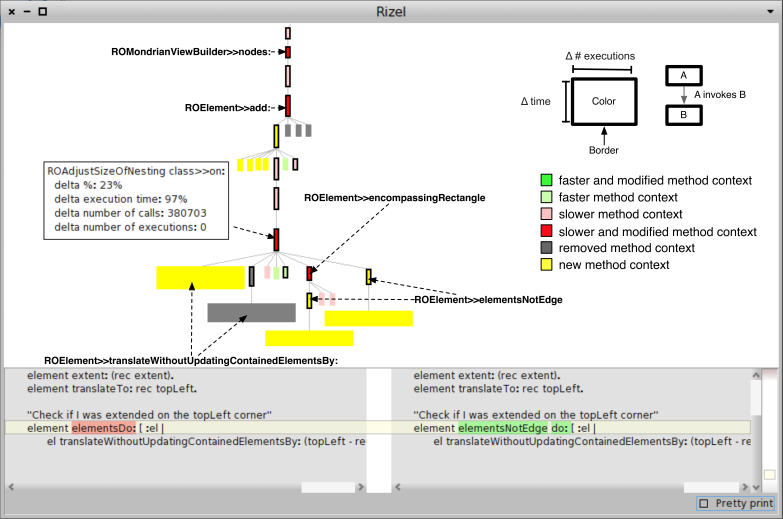
\includegraphics[scale=0.58]{Imagens/trabalho_relacionado_performance_evolution_blueprint.png}}
   \textsf{\caption[Exemplo do \textit{Performance Evolution Blueprint}]{Exemplo do \textit{Performance Evolution Blueprint} \cite{SandovalAlcocer2013}.\label{fig:trabalhos-relacionados-performance-evolution-blueprint}}}
\end{figure}

A ferramenta {\textit{\toolName}} e o \textit{Performance Evolution Blueprint} utilizam a metáfora de grafo, no entanto, a primeira oferece as seguintes vantagens com relação à segunda:
\begin{itemize}
   \item \textit{Informações da Hierarquia de Chamadas}: diferentemente do \textit{Performance Evolution Blueprint}, o grafo de chamadas do {\textit{\toolName}} mostra informações adicionais como o tempo de execução total, próprio e de desvio para cada nó, o tempo de execução do cenário, os nomes de cada nó da hierarquia de chamadas (próximos ao nó desviado/adicionado/removido) e os parâmetros dos métodos. O \textit{Performance Evolution Blueprint}, além de exibir informações comuns ao {\textit{\toolName}} como a porcentagem de desvio de desempenho, mostra informações diferentes como os métodos que tiveram degradações de desempenho mas não foram alterados. As informações apresentadas pela ferramenta {\textit{\toolName}} se mostram bastante úteis, como mencionado pelo participante P5GA do estudo conduzido e apresentado nesta dissertação: \textit{``o gráfico é bastante simples e fácil de entender. Não há muita informação, apenas o necessário.''}. Soma-se a isso, o conteúdo contido na seção de Sumário e Histórico da visualização. Com essas informações, torna-se factível identificar não só as possíveis causas dos desvios de desempenho, mas também a sua gravidade e localização na hierarquia de chamadas;
   \item \textit{Diferentes Elementos Visuais}: a visualização do grafo de chamadas do {\textit{\toolName}} fornece elementos visuais diferentes para exibir as informações. O nó de agrupamento mostra que existem mais nós que foram omitidos e não estão diretamente ligados aos indicados com desvios/adicionados/removidos. Na visualização proposta por \citeauthor{SandovalAlcocer2013}, esses nós são, por padrão, omitidos, mas podem ser exibidos através da interação do usuário. Outro elemento visual são as setas indicativas da porcentagem de degradação ou otimização dos nós, propiciando a identificação da gravidade do desvio de cada nó. Esse elemento visual foi mencionado no estudo, pelo participante P5GA: \textit{``Eu gostei .. da seta verde/vermelha indicando o nível de melhoria/degradação.''}. No \textit{Performance Evolution Blueprint}, ao passar o mouse sobre um nó, o usuário pode ter acesso a informações como as porcentagens de desvio desse nó, nome da classe e do método e a diferença da quantidade de execuções da versão anterior para a atual. Dessa forma, não há uma visão geral da gravidade do desvio de todos os nós indicados com variações de desempenho;
   \item \textit{Diferentes Funcionalidades}: o grafo de chamadas do {\textit{\toolName}} possui funcionalidades de zoom e destaque da hierarquia de chamada dos nós com desvio/adicionados/removidos;
   \item \textit{Maior Potencial de Aplicabilidade}: por ser compatível com a linguagem de programação Java, o potencial de aplicabilidade da ferramenta proposta por esta dissertação é maior. Para efeitos comparativos, no momento da escrita deste trabalho, existem no GitHub mais de 3 milhões e 300 mil projetos \textit{open source} implementados na linguagem Java, ao passo que na linguagem SmallTalk existem pouco mais de 2 mil;
   \item \textit{Avaliação com Participantes}: a avaliação com participantes realizada nesta dissertação é um diferencial com relação ao trabalho de \citeauthor{SandovalAlcocer2013}. A partir dessa avaliação foi possível obter valiosas respostas dos usuários com relação a utilidade das visualizações para identificação das possíveis causas de variações de desempenho e a sua aplicabilidade nos processos de desenvolvimento de software das equipes.
\end{itemize}

%O trabalho proposto se diferencia do de \citeauthor{SandovalAlcocer2013} pelo fato de: (i) ser compatível com a linguagem Java; (ii) mostrar mais informações sobre a hierarquia de chamadas; (iii) exibir a evolução de cada cenário entre as versões do softwares; e (iv) utilizar diferentes elementos visuais para destacar a evolução do desempenho na visualização do \textit{call graph} dos cenários.

\citeauthor{Bergel} propuseram uma abordagem cujo objetivo é comparar duas versões de um software para a identificação de gargalos de execução. As visualizações propostas foram \textit{Structural Distribution Blueprint} e \textit{Behavioral Distribution Blueprint}. Ambas exibem informações de execução como um \textit{call graph}, onde os nós são os métodos e as arestas são as invocações. Cada nó é renderizado como uma caixa e uma invocação é uma linha que une dois nós. A primeira visualização exibe uma métrica que indica a distribuição do tempo de execução ao longo da estrutura estática de um programa. Já a segunda mostra as informações de tempo de execução junto com as chamadas de métodos. Essa abordagem considera apenas se um método gastou ou não mais tempo de execução do que na versão anterior. A Figura \ref{fig:trabalhos-relacionados-bergel-robbes-binder} exemplifica a visualização proposta pelos autores. A avaliação foi realizada ao aplicar a ferramenta no \textit{framework} Mondrian\footnote{\href{http://scg.unibe.ch/archive/papers/Meye06aMondrian.pdf}{http://scg.unibe.ch/archive/papers/Meye06aMondrian.pdf}}.

As principais vantagens do trabalho proposto por esta dissertação com relação ao de \citeauthor{Bergel} são:
\begin{itemize}
   \item \textit{Mais Métricas}: por adicionar mais métricas no grafo de chamadas, como a porcentagem de desvio de desempenho e se houve métodos adicionados ou removidos, o {\textit{\toolName}} fornece a possibilidade de o usuário identificar as possíveis causas e a gravidade dos desvios de desempenho. Essas métricas adicionadas fortalecem a análise da evolução do sistema ao longo das versões;
   \item \textit{Agrupamento de Nós}: no {\textit{\toolName}}, o nó de agrupamento mostra que existem mais nós na hierarquia de chamadas que foram omitidos e não estão diretamente ligados aos indicados com desvios/adicionados/removidos. A proposta de \citeauthor{Bergel} não menciona sobre a escalabilidade em nenhuma das suas visualizações, nem como essa situação é tratada;
   \item \textit{Identificação das Causas dos Desvios}: o grafo de chamadas do {\textit{\toolName}} indica os \textit{hashes} dos \textit{commits} que possivelmente foram os responsáveis pelos desvios de desempenho dos nós e, consequentemente, do cenário. As visualizações \textit{Structural Distribution Blueprint} e \textit{Behavioral Distribution Blueprint} não fornecem essa possibilidade;
   \item \textit{Verificação das Mudanças}: outra vantagem é que, uma vez que os \textit{hashes} dos \textit{commits} são exibidos para os nós com desvios/adicionados/removidos, eles podem ser clicados e, assim, o usuário tem acesso às mudanças implementadas no código-fonte que podem ter causado tal desvio de desempenho;
   \item \textit{Visão Geral dos Cenários}: \citeauthor{Bergel} não mencionam se há uma forma de se obter uma visão geral dos gargalos de desempenho, para duas versões de um software, encontrados pela abordagem. Para essa finalidade, o {\textit{\toolName}} fornece a visualização de sumarização de cenários.
\end{itemize}

\begin{figure}[!htb]
   \centering
   \frame{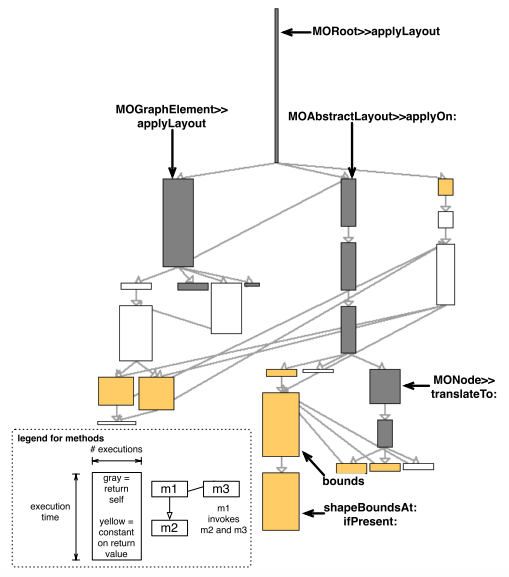
\includegraphics[scale=0.60]{Imagens/trabalho_relacionado_bergel_robbes_binder.png}}
   \textsf{\caption[Exemplo da visualização comportamental proposta por Bergel, Robbes e Binder.]{Exemplo da visualização comportamental proposta por \citeauthor{Bergel}.\label{fig:trabalhos-relacionados-bergel-robbes-binder}}}
\end{figure}

\citeauthor{Mostafa2009} propõem uma técnica que compara duas árvores de contexto de chamadas \abrv[CCT -- \textit{Context Call Tree}]{}(CCT, do inglês \textit{Context Call Tree}), cada uma obtida de uma versão diferente de um software. Os autores apresentam o \textit{PARCS}, uma ferramenta de análise que identifica automaticamente diferenças entre o comportamento da execução de duas revisões de uma aplicação. A abordagem usa como base o algoritmo de correspondência de árvores comuns para comparar duas CCTs. No entanto, o suporte visual usado pelo PARCS não representa adequadamente a variação de uma estrutura dinâmica e múltiplas métricas \cite{Pablo2013}. Outra limitação dessa abordagem é que ela não detecta nós adicionados. Quando comparadas, duas CCTs que diferem apenas em um nó adicionado são consideradas completamente diferentes pelo PARCS. A Figura \ref{fig:trabalhos-relacionados-parcs} exibe um exemplo das diferenças topológicas encontradas entre duas versões do FindBugs\footnote{\href{http://findbugs.sourceforge.net}{http://findbugs.sourceforge.net}}, ferramenta utilizada para a avaliação da abordagem. Na figura, no centro dos nós são mostrados os seus ids, os nós retangulares representam métodos modificados e os nós em cinza indicam CCTs diferentes com relação à versão anterior.

\begin{figure}[!htb]
   \centering
   \frame{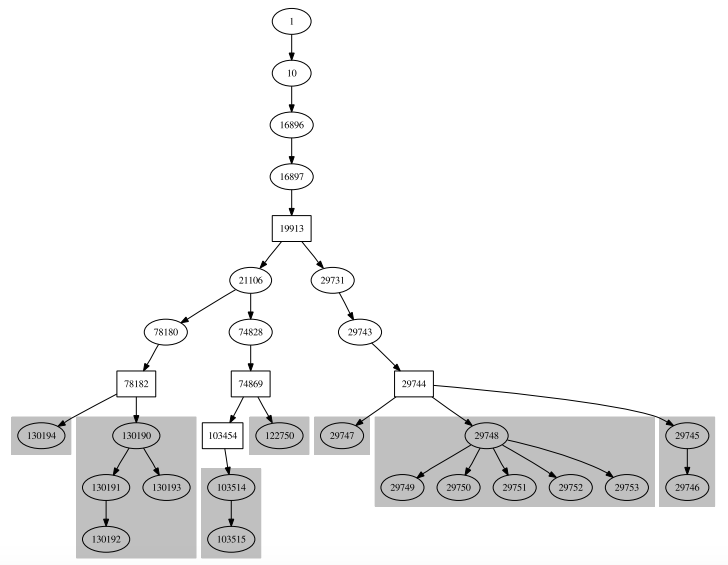
\includegraphics[scale=0.60]{Imagens/trabalho_relacionado_parcs.png}}
   \textsf{\caption[Exemplo do PARCS.]{Exemplo do PARCS \cite{Mostafa2009}.\label{fig:trabalhos-relacionados-parcs}}}
\end{figure}

O trabalho proposto nesta dissertação oferece as seguintes vantagens ao PARCS, dentre outras:
\begin{itemize}
   \item \textit{Nós Adicionados e Removidos}: o grafo de chamadas do {\textit{\toolName}} destaca os nós adicionados e removidos na hierarquia de chamadas de cada cenário. Esses nós são fundamentais para o entendimento da real causa dos desvios de desempenho de determinado cenário ao longo das versões;
   \item \textit{Mais Métricas}: de maneira semelhante ao trabalho relacionado comentado anteriormente, por adicionar mais métricas no grafo de chamadas, como a porcentagem de desvio de desempenho, os tempos de execução total, próprio e de desvio para cada nó, o {\textit{\toolName}} fornece a possibilidade de o usuário identificar as possíveis causas e a gravidade dos desvios de desempenho;
   \item \textit{Identificação das Causas dos Desvios}: diferentemente do trabalho de \citeauthor{Mostafa2009}, o grafo de chamadas do {\textit{\toolName}} indica os \textit{hashes} dos \textit{commits} que possivelmente foram os responsáveis pelos desvios de desempenho dos nós e, consequentemente, do cenário;
   \item \textit{Verificação das Mudanças}: por indicar os \textit{hashes} dos \textit{commits}, ao clicar nesses \textit{hashes}, o usuário pode ter acesso às mudanças implementadas no código-fonte que podem ter causado o desvio de desempenho do cenário;
   \item \textit{Visão Geral dos Cenários}: os autores não mencionam se há uma forma de se obter uma visão geral das comparações entre as revisões da aplicação. A visualização da sumarização de cenários fornecida pelo {\textit{\toolName}} possibilita ao usuário obter uma visão geral de todos os cenários para a análise de um par de versões de um software.
\end{itemize}

\citeauthor{Bezemer2015} realizam a comparação do desempenho de duas versões de um software através de gráficos de chama diferenciais (do inglês, \textit{differential flame graphs} -- DFG). Dadas duas versões \textit{v1} (anterior) e \textit{v2} (atual), a ferramenta realiza a comparação de três maneiras: (i) com \textit{v1} como base, (ii) com \textit{v2} como base e (iii) apenas as diferenças do item (ii). Eles utilizam cores para destacar as comparações: o branco indica que não houve mudanças, o azul que houve melhora no desempenho e o vermelho indica que este piorou. Entretanto, a abordagem não indica as causas das variações de desempenho e os autores indicam que o principal desafio é a coleta dos dados, pois são necessárias ferramentas de \textit{profiling} de terceiros para a análise das versões e eles destacam que pode ser difícil coletar os dados para algumas linguagens, como o Java e Python. A Figura \ref{fig:trabalhos-relacionados-dfg} mostra um exemplo de DFG para o software utilitário Rsync\footnote{\href{https://rsync.samba.org}{https://rsync.samba.org}}, utilizado na avaliação da abordagem. A figura exibe a pilha de chamadas dos métodos onde a largura de cada elemento indica o seu tempo de execução. Os elementos em branco representam os métodos que não tiveram alterações no seu desempenho, já os indicados em vermelho são os que tiveram seu desempenho degradado entre as versões. O método exibido em um tom mais escuro de vermelho indica que a variação de desempenho foi maior do que o método exibido em um tom mais claro.

\begin{figure}[!htb]
   \centering
   \frame{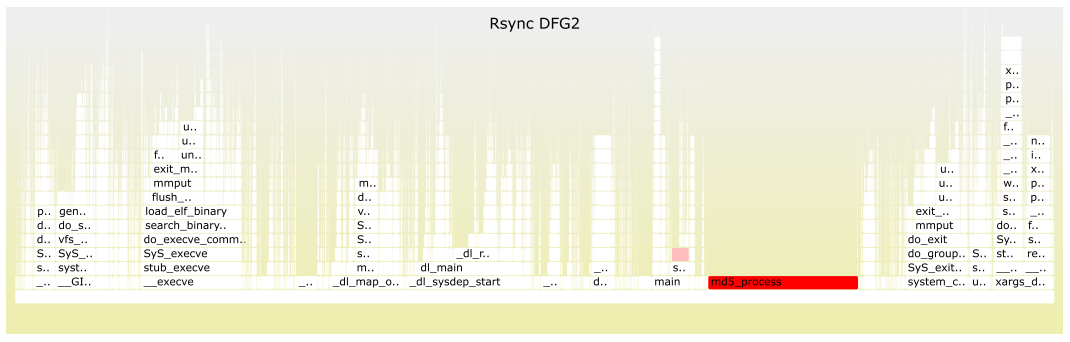
\includegraphics[scale=0.42]{Imagens/trabalho_relacionado_dfg.png}}
   \textsf{\caption[Exemplo do DFG.]{Exemplo do DFG \cite{Bezemer2015}.\label{fig:trabalhos-relacionados-dfg}}}
\end{figure}

O {\textit{\toolName}} apresenta vantagens com relação ao DFG, embora as metáforas visuais utilizadas sejam diferentes:
\begin{itemize}
   \item \textit{Mais Métricas}: o DFG apresentado pelos autores apresentam poucas métricas com relação aos métodos executados. O trabalho proposto por esta dissertação mostra os tempos de execução total, próprio e o desvio para cada nó, a porcentagem do desvio, apresenta mais claramente os nomes dos nós na hierarquia de chamadas, além das informações que constam nas seções de Sumário e Histórico da visualização;
   \item \textit{Nós Adicionados e Removidos}: o {\textit{\toolName}} destaca os nós adicionados e removidos na hierarquia de chamadas de cada cenário, diferentemente do DFG. Como comentado anteriormente, a identificação desses nós são fundamentais para o entendimento da real causa dos desvios de desempenho de determinado cenário ao longo das versões;
   \item \textit{Agrupamento de Nós}: no {\textit{\toolName}}, o nó de agrupamento mostra que existem mais nós na hierarquia de chamadas que foram omitidos e não estão diretamente ligados aos indicados com desvios/adicionados/removidos. O DFG mostra todo rastreamento da pilha de chamadas dos métodos, de modo que se essa pilha for extensa, torna-se muito difícil, ou até mesmo inviável, identificar e distinguir os seus elementos;
   \item \textit{Identificação das Causas dos Desvios}: diferentemente do trabalho de \citeauthor{Bezemer2015}, o {\textit{\toolName}} indica os \textit{hashes} dos \textit{commits} que possivelmente foram os responsáveis pelos desvios de desempenho dos nós e, consequentemente, do cenário;
   \item \textit{Verificação das Mudanças}: por indicar os \textit{hashes} dos \textit{commits}, ao clicar nesses \textit{hashes}, o usuário pode ter acesso às mudanças implementadas no código-fonte que podem ter causado o desvio de desempenho do cenário;
   \item \textit{Visão Geral dos Cenários}: Os autores não mencionam se, através da abordagem, é possível obter uma visão geral das comparações realizadas. A visualização da sumarização de cenários fornecida pelo {\textit{\toolName}} possibilita uma visão geral de todos os cenários para a análise de um par de versões de um software.
\end{itemize}